%%%%%%%%%%%%%%%%%%%%%%%%%%%%%%%%%%%%%%%%%
% University/School Laboratory Report
% LaTeX Template
% Version 3.1 (25/3/14)
%
% This template has been downloaded from:
% http://www.LaTeXTemplates.com
%
% Original author:
% Linux and Unix Users Group at Virginia Tech Wiki
% (https://vtluug.org/wiki/Example_LaTeX_chem_lab_report)
%
% License:
% CC BY-NC-SA 3.0 (http://creativecommons.org/licenses/by-nc-sa/3.0/)
%
%%%%%%%%%%%%%%%%%%%%%%%%%%%%%%%%%%%%%%%%%

%----------------------------------------------------------------------------------------
%	PACKAGES AND DOCUMENT CONFIGURATIONS
%----------------------------------------------------------------------------------------

\documentclass{article}

\usepackage{float} % Required for images to be placed inline
\usepackage[version=3]{mhchem} % Package for chemical equation typesetting
\usepackage{siunitx} % Provides the \SI{}{} and \si{} command for typesetting SI units
\usepackage{graphicx} % Required for the inclusion of images
\usepackage{natbib} % Required to change bibliography style to APA
\usepackage{amsmath} % Required for some math elements

\setlength\parindent{0pt} % Removes all indentation from paragraphs

\renewcommand{\labelenumi}{\alph{enumi}.} % Make numbering in the enumerate environment by letter rather than number (e.g. section 6)

%\usepackage{times} % Uncomment to use the Times New Roman font

%----------------------------------------------------------------------------------------
%	DOCUMENT INFORMATION
%----------------------------------------------------------------------------------------

\title{Coulomb's Law Lab\\ PHY-222-AC01} % Title

\author{Jasper \textsc{Runco}} % Author name

\date{\today} % Date for the report

\begin{document}

\maketitle % Insert the title, author and date

\begin{center}
	\begin{tabular}{l r}
	\end{tabular}
\end{center}

% If you wish to include an abstract, uncomment the lines below
% \begin{abstract}
% Abstract text
% \end{abstract}

%----------------------------------------------------------------------------------------
%	SECTION 1
%----------------------------------------------------------------------------------------

\section{Theory}

Coulomb's law describes a mathematical expression for the interaction of electrically charged objects.
The electrical charge generates a force pair, $F_{E}$, with a magnitude that has been experimentally determined
to such a degree that it is accepted as a universal law.

\subsection{Definitions}
\label{definitions}
\begin{description}
	\item[Electrically charged object -]
		Matter with more or less electrons than protons is negatively or
		positively charged respectively.
	\item[Force pair -]
		The principal of Newton's third law in which every action force has a corresponding reaction force
		equal in magnitude and opposite in direction.
	\item[Coulomb's law -]
		\[F_{E} = k \frac{q_1 q_2}{r^2}\]
		\begin{description}
			\item[r -]
				The distance between the charged objects measured in meters.
			\item[$q_1 q_2$ -]
				The sum of the electrical charges of each object, measured in Coulombs.
			\item[k -]
				The electric constant, the experimentally determined proportionality constant with a value
				of $k = 9.0 \times 10^{9} \frac{Nm^2}{C^2}$

		\end{description}
\end{description}

%----------------------------------------------------------------------------------------
%	SECTION 2
%----------------------------------------------------------------------------------------
\section{Objectives}


% If you have more than one objective, uncomment the below:
\begin{description}
	\item[First Objective] \hfill \\
		Experimentally confirm Coulomb's law.
	\item[Second Objective] \hfill \\
		Study how distance and charge affect the electric force.
	\item[Third Objective] \hfill \\
		Experimentally determine the value of the electric constant, k.
\end{description}


%----------------------------------------------------------------------------------------
%	SECTION 3
%----------------------------------------------------------------------------------------

\section{Experimental Data}

\subsection{Part One}%
\label{sub:part_one}


\begin{table}[htpb]
	\centering
	\caption{}
	\label{tab:label}
	\begin{tabular}{| c |  c | c |  c | }
		\hline
		$q_1= 2 \mu C$ & &  $q_2 = 4 \mu C$  &\\
		\hline
		\textbf{r(cm)} & \textbf{$r^2(m^2)$} & $\frac{1}{r^2}(\frac{1}{m^2})$ & $F_{E}(N)$ \\
		\hline
		10 & $1.0 \times 10^{-2}$ & $1\times 10^{2}$& $7.190$ \\
		\hline
		9 & $8.1 \times  10^{-3}$& $1.2 \times 10^{2}$ & $8.877$\\
		\hline
		8 & $6.4 \times 10^{-3}$& $1.6 \times 10^{2}$ & $11.234$\\
		\hline
		7 & $4.9 \times  10^{-3}$& $2.0 \times  10^{2}$ & $14.674$ \\
		\hline
		6 & $3.6 \times 10^{-3}$& $2.8 \times 10^{2}$& $19.972$\\
		\hline
		5 & $2.5 \times 10^{-3}$ & $4.0 \times  10^2$& $28.760$ \\
		\hline
		4 & $1.6 \times  10^{-3}$& $6.3 \times  10^2$ & $44.938$ \\
		\hline
		3 & $9.0 \times  10^{-4}$& $1.1 \times  10^{3}$ & $ 79.889$\\
		\hline
	\end{tabular}
\end{table}

\subsection{Part Two}%
\label{sub:part_two}

\begin{table}[htpb]
	\centering
	\caption{}
	\label{tab:label}
	\begin{tabular}{| c | c |}
		\hline
		$q_1 = 5 \mu C$ & $ r = 6 cm$   \\
		\hline
		$q_2 (\mu C)$ & $F_{E}(N)$\\
		\hline
		10 & $124.827$  \\
		\hline
		9 &  $112.344$ \\
		\hline
		8 &  $99.862$ \\
		\hline
		7 &  $87.379$ \\
		\hline
		6 &   $74.896$\\
		\hline
		5 &  $62.414$ \\
		\hline
		4 &   $49.931$\\
		\hline
		3 &  $37.448$ \\
		\hline
	\end{tabular}
\end{table}


%----------------------------------------------------------------------------------------
%	SECTION 4
%----------------------------------------------------------------------------------------

\section{Data Analysis}

\subsection{Part One}%
\label{sub:part_one}


\subsubsection{$F_{E}$ with respect to $r$}%
\label{ssub:_f__e_with_respect_to_r_}

\begin{figure}[H]
	\begin{center}
		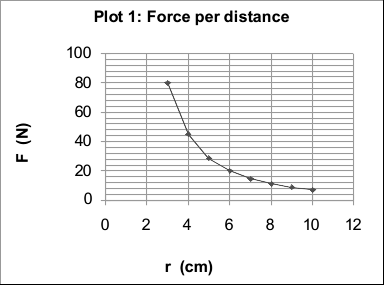
\includegraphics[width=0.65\textwidth]{plot1} % Include the image placeholder.png
		\caption{Force per distance}
	\end{center}
\end{figure}

\begin{description}
	\item[Comments on Figure 1:] As the charged objects' distance $(r)$ tends towards zero
		from the possitive direction, the force $(F)$ tends towards infinity. As $r$ tends
		towards positive infinity, $F$ tends towards zero.
\end{description}

\subsubsection{$F_{E}$ with respect to $\frac{1}{r^2}$ to find $k$}%

\begin{figure}[H]
	\begin{center}
		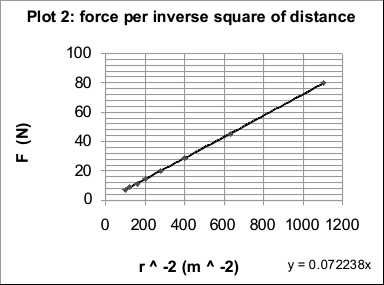
\includegraphics[width=0.65\textwidth]{plot2} % Include the image placeholder.png
		\caption{Force per inverse square of distance}
	\end{center}
\end{figure}


\begin{description}
	\item[Coulomb's Law -]
		$F_{E} = k \frac{q_1 q_2}{r^2}$
	\item[Linear regression of Figure 2 data -] y = 0.072238x
	\item[$q_1$ -] $2 \mu C$
	\item[$q_2$ -] $4 \mu C$
\end{description}

\begin{align*}
	F_{E} &= k \frac{(2 \mu C)(4 \mu C)}{r^2} \implies \\
	F_{E} (N) &= k \left( 8 \times 10^{-12} C^2 \right)  \left( \frac{1}{r^2} \right) \left( \frac{1}{m^2} \right)  \\
	y &= 0.072238x \implies \\
	F_{E} &= 0.072238 \left( \frac{1}{r^2} \right)  \\
	0.072238 \left( \frac{1}{r^2} \right) (N) &=  k \left( 8 \times 10^{-12} C^2 \right) \left( \frac{1}{r^2} \right) \left( \frac{1}{m^2} \right)\\
	k &= \frac{  0.072238 \left( \frac{1}{r^2} \right) (N)(m^2)}{8 \times 10^{-12} C^2 \left(  \frac{1}{r^2}\right)  } \\
	k &= \boxed{9.02975 \times 10^{9}}\left( \frac{N m^2}{C^2} \right)  \\
\end{align*}


\subsubsection{Percent error in $k$}%
\label{ssub:percentag}

\begin{align*}
	\:\text{\% error}\: &= \left| \frac{\:\text{theoretical}\: - \:\text{experimental}\:}{\:\text{theoretical}\:}  \right| \times 100\%\\
\:\text{\% error}\: &= \left|   \frac{\left( 9.0 \times 10^{9} \frac{N m^2}{C^2} \right) - \left( 9.02975 \times 10^{9}\frac{N m^2}{C^2}  \right) }{\left( 9.0 \times 10^{9} \frac{N m^2}{C^2} \right)} \right| \times 100\%\\
\:\text{\% error}\: &= 0.330556 \%
\end{align*}



\subsection{Part Two}%
\label{sub:part_two}



\subsubsection{$F_{E}$ with respect to $q_{2}$}%
\label{ssub:_f__e_with_respect_to_q__2_}

\begin{figure}[H]
	\begin{center}
		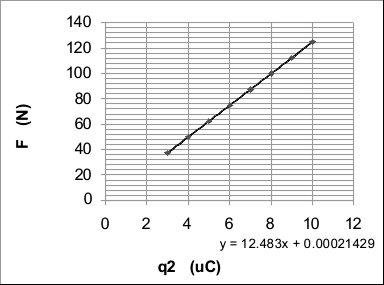
\includegraphics[width=0.65\textwidth]{plot3} % Include the image placeholder.png
		\caption{Force per magnitude charge on $q_{2}$}
	\end{center}
\end{figure}



\begin{description}
	\item[Comments on Figure 3: ]
		There is a positive linear relationship between the magnitude of charge on one object $q_2 (\mu C)$ and
		electric force $F_{E} (N)$. Given the precision of $F_{E}$ measurement, it appears to approach a
		lower bounds of $F_{E} = 0$ at $q_2 = 0$.
\end{description}



\subsubsection{$F_{E}$ with respect to $q_2$ to find $k$}%
\label{ssub:_f__e_with_respect_to_q_2_to_find_k_}


\begin{description}
	\item[Coulomb's Law -]
		$F_{E} = k \frac{q_1 q_2}{r^2}$
	\item[Linear regression of Figure 3 data -] $y = 12.483 x + 0.00021429$
	\item[$q_1$ -] $5 \mu C$
		\item[r -] $6 cm$
\end{description}

\begin{align*}
	F_{E} &= k \frac{(5 \mu C)(q_2)}{(6cm)^2} \implies \\
	F_{E}(N) &=  k q_2(\mu C) \left( \frac{5\times 10^{-6}C}{3.6 \times 10^{-3}m^2} \right)  \\
	y &= 12.483 x + 0.00021429 \implies \\
	F_{E} &= 12.483 q_2 + 0.00021429 \\
	(12.483 q_2 + 0.00021429) (N) &=  k q_2(\mu C) \left( \frac{5\times 10^{-6}C}{3.6 \times 10^{-3}m^2} \right) \implies \\
	k &= \frac{ (12.483 q_2 + 0.00021429)(3.6\times 10^{-3} m^2)(N)}{(q_2)(5\times 10^{-6}C)(10^{-6}C)} \implies  \\
	k &=  \boxed{ 8.98776 \times 10^{9} \left( \frac{Nm^2}{C^2} \right)}  + 1.542888 \times 10^{5}q_2^{-1}\left( \frac{Nm^2}{C^2} \right) \\
\end{align*}


\subsubsection{Percent error in $k$}%
\label{ssub:percentag}

\begin{align*}
	\:\text{\% error}\: &= \left| \frac{\:\text{theoretical}\: - \:\text{experimental}\:}{\:\text{theoretical}\:}  \right| \times 100\%\\
\:\text{\% error}\: &= \left|   \frac{\left( 9.0 \times 10^{9} \frac{N m^2}{C^2} \right) - \left( 8.98776 \times 10^{9}\frac{N m^2}{C^2}  \right) }{\left( 9.0 \times 10^{9} \frac{N m^2}{C^2} \right)} \right| \times 100\%\\
\:\text{\% error}\: &= 0.136 \%
\end{align*}


%----------------------------------------------------------------------------------------
%	SECTION 5
%----------------------------------------------------------------------------------------

\section{Results and Conclusions}




%----------------------------------------------------------------------------------------
%	SECTION 6
%----------------------------------------------------------------------------------------

\section{Discussion of Experimental Uncertainty}



\end{document}
